\onehalfspacing
\label{chapter3}
\section{A Working Definition of Flow}

In comparison to its conceptual counterpart ``the beat'', a ``flow'' resists a clear 
definition in academic and technical discourse. While there seems to be some agreement
that the beat is comprised of musically-distinct layers looping throughout a piece, 
definitions of flow range from anywhere as specific as ``simply the rhythms and rhymes
[a hip-hop song] contains''\footnote{
    \autocite[63]{pauledwardsHowRapArt2009}. While Edwards' statement comes within the 
    context of an instruction on rapping (and therefore his reductiveness may be 
    pedagogically useful), this attitude toward flow is implied by music academics who 
    transcribe flow primarily on one line of staff notation; such transcriptions implicitly
    show flow as something existing within a fixed (or indiscernible) pitch space, with 
    unambiguous, highly discernible rhythms.} 
to as wide-ranging as ``all of the rhythmical and articulative features of an emcee's 
delivery of the lyrics.''\footnote{
    \cite{kyleadamsMetricalTechniquesFlow2009}.} 
Before I name and discuss a few of the stylistic hallmarks of flow in underground hip-hop,
it will be worthwhile for me to construct a definition that ascertains what musical elements
comprise it.

Consider, once more, Open Mike Eagle's characterization of his own relationship to MF 
DOOM's flow: that Eagle has to be careful with it because of how much time he has spent
`in DOOM's mind.'\footnote{
    \cite{estellecaswellRappingDeconstructedBest2016}. For my earlier discussion of this
    passage and its relationship to meditative listening,  see Section~\ref{listeningasmeditation}.} 
The fact that Eagle can characterize his relationship to the style of DOOM's flow demonstrates
that flow encompasses more than rhythm and rhyme alone; by themselves these elements do not
account for flow as being tied to an emcee's specific or generic style. Flow, then, should
be conceived more broadly than the manifestation of rhythms through the vocal delivery of
rhymes.

At the same time, emcees frequently describe flow as text in relation to the music, drawing 
contrasts with the non-musically bounded epithet ``poetry.'' The emcee Rakim's oft-cited 
definition of rap (that it is ``rhythm and poetry'') creates a distinction between texts that
can be rapped and those that are conceived within the poetic medium. Clarifying this distinction,
the emcee Myka 9 of Freestyle Fellowship offers, ``sometimes I might write a poem, a spoken-word
poem, but then morph that into a rap rhythmically.''\footnote{
    \autocite[63]{pauledwardsHowRapArt2009}.}
Myka 9's insight helps to construct a continuum for rapped text: it exists on a spectrum from 
texts that are spoken in musically-bounded ways and non-musically-bounded ways.\footnote{
    Interestingly, rapped verses can be and often are delivered on varying degrees of this
    spectrum. Mitchell Ohriner notes two distinct modes of delivery, which he calls speech-rhythmic
    and music-rhythmic, based on the degree of non-alignment between the musical meter and the 
    degree to which syllable onsets correspond to metrical positions (see 
    \cite{mitchellohrinerLyricRhythmNonalignment2019}.}

This distinction between the rap's structure as text and its performance as music is 
foundational to the method by which I interrogate the concept of flow in this chapter. 
I believe the techniques underground emcees employ when rapping can be divided into 
categories I refer to as \emph{structural} and \emph{performance} techniques. Structural
techniques deal primarily with rap as text, considering its syntactic elements with 
primacy  over their manifestation as a stream in the musical object. By contrast, 
performance techniques focus on rap as music, considering the ways in which an emcee 
makes manifest the structures they contrive when composing texts. Performance techniques
also encapsulate the decisions made when treating the voice as an object within a 
digital recording. With these categories, I aim to examine how, as Mitchell Ohriner 
claims, flow ``encompasses phrasing, rhythm, meter, accent, patterning, and groove, not
to mention the relations among these parameters.''\footnote{
    \autocite[28]{mitchellohrinerFlowRhythmicVoice2019}.}

\section{Thesis Statement \& Definitions}

In this chapter, I examine a few notable techniques that underground emcees employ 
in structuring and performing their flow; I argue that, like producers, their choice
to use these techniques reaches listeners as underground. The four techniques I define
below do not form an exhaustive list, but rather are salient and illustrative in how 
they relate to my conception of the subgenre. My terms are also  divided into the 
subcategories of structural and performance techniques, a distinction I draw in my 
understanding of how emcees work with the text that makes up their flow. When the 
underground emcee inhabits the role of writer, they experiment with structuring 
techniques including \emph{pivot rhyme} and \emph{closing fragmentation} to craft 
their verses. Stepping into the recording booth or onto the stage, the emcee shifts
into their role as rapper and therefore draws on performance techniques such as 
\emph{mimesis} and \emph{processing} to shape their vocal delivery. Each of these 
techniques serves as the focus of one of the close-readings that follow, so I will
clarify their functions before provide examples.

As a device for constructing a verse, a pivot rhyme allows an emcee to execute a shift 
in end rhyme; it occurs when the concluding words of the previous bar conjure up an idea
that is semantically linked  to the bar's topic but does not rhyme. In this instance, the
rapper chooses to displace the lyric past the next bar line, allowing that word or phrase 
to serve as the primary rhyming sound within a new repetition of the beat pattern. Often 
the emcee uses this instance as a way to play with audience expectation, taking the listener's
focus on this final rhyme to shift towards a topic semantically distinct from the previous bar.

Underground emcees employ closing fragmentation as another method of structuring a verse, 
particularly to mark the end of some sort of formal section. To accomplish this, emcees will
deliver a ``full'' textual phrase, usually structured as a setup and punchline, then signal 
a close through breaking up and repeating the component elements of that textual phrase in a 
more improvisatory and loosely-organized style of delivery. Fragmentation and repetition here 
do not function as they do in the construction of a hook; rather, they demonstrate to the 
listener that some larger textual unit\textemdash a phrase, a verse, the song itself\textemdash
is ending.

With both performance techniques, emcees articulate the role of their voice as a layer
\emph{amongst} the rest of the mix, rather than the principal element within it. In particular,
the use of mimesis, or stylizing vocal delivery to mimic other elements in the beat layer, 
draws attention to the other musical elements in an attempt to foreground their musicality.
This promotes the other musical layer to a co-soloist role, rather than functioning as a
background loop or layer, allowing the listener to focus on it as more than just 
accompanimental structure beneath the vocal flow.

Processing more generally refers to the manipulation of digital audio after it is recorded
(especially through the use of EQ, compression, and reverb software or hardware), but here 
I use it to refer to methods of altering the vocal signal as a form of electronic composition.
In particular, rappers use processing effects like delay, distortion, and pitch transposition
to alter the audio of their voice during or after tracking it to treat it as a musically 
manipulable element; the vocals here function as \emph{sound} as much as they do 
text.\footnote{
    My definition of processing here is a broader version of the definition of ``glitch'' 
    in Chapter 2 (see p.~\pageref{glitch}.)}
In this way, processing treats the voice as if it were any other musical layer and, as a 
result, any layer can be listened with as much consideration as the voice.

%clearpage
\section{Structuring Techniques}
The transcription of flow makes clear the limitations of staff notation, perhaps more than
transcription of any other musical element. Throughout this project, my dedication to 
transcription in standard notation arises from my desire to emulate what Kofi Agawu 
conceptualizes as a ``post  colonial transcription,'' one based in an ``ideology of 
sameness so that\textellipsis we can gain a better view of difference.''\footnote{
    \autocite[67]{kofiagawuInventionAfricanRhythm2003}. Agawu's chapter traces a history of 
    non-African scholars transcribing Northern Ewe drumming in a way that both essentializes
    and exoticizes African music as primarily rhythmic and therefore fundamentally different
    from Western approaches to music making. Although I do not wish to employ colonization 
    uncritically as a metaphor for music theory's relationship to hip-hop, I do believe that
    the same essentializing and exoticizing tendencies would manifest if I were to completely
    avoid standard notation for this repertory.}
However, this approach exists at odds with another point noted by Agawu: no singular mode
of representation can sufficiently convey the totality of a musical listening 
experience.\footnote{
    \autocite[187]{kofiagawuAfricanRhythmNorthern1995}.}
In dealing with flow as a textual structure independent from its musical manifestation, 
I will opt to use another mode of representation: namely, Ohriner's $modulo$ 16 grid 
transcriptions.\footnote{
    For a detailed overview of the system and a few sample transcriptions, see 
    \autocite[xxviii--xl, 7--9]{mitchellohrinerFlowRhythmicVoice2019}.}

Ohriner's method of transcription simplifies certain elements that become problematic
when transcribing flow in standard notation. First, his 16-point grid for a bar avoids
proliferate use of eighth, sixteenth, and thirty-second notes, not to mention syncopation
between them. Subsequently, his method also simplifies the naming structure by labeling 
each metric position with a number from 0--15; one can more succinctly communicate a 
syllable landing on ``the third sixteenth note of beat 3'' as position 10, for instance. 
Finally, Ohriner's system does not force a transcriber to choose fixed metrical positions
in the same way standard notation and adaptations of TUBS for flow do; if a syllable onset
occurs slightly before the beat, this can be accounted for simply by moving the corresponding
circle. Although vocal groove and non-alignment with the meter is not a focus in this chapter,
the ability for a system to adapt between quantized and non-quantized rhythms is foundational
to being able to transcribe flow.

\phantomsection
\subsection*{\centering Madvillain's ``Great Day''}
\addcontentsline{toc}{subsection}{Madvillain's ``Great Day''}

Madvillain, the moniker under which DOOM and Madlib released all of their collaborations
except for ``One Beer,'' looms large in the world of underground hip-hop. One unrelenting 
focus of the accolades for  their 2004 double LP \textit{Madvillainy} is DOOM's flow: in 
the words of Ta-Nehisi Coates, ``[\textit{Madvillainy}'s] singular sound came mostly from
[DOOM's] raspy baritone rendering a sort of nerdcore poetry.''\footnote{
    \cite{ta-nehisicoatesMaskDoomNonconformist2009}.}

This claim to DOOM's uniqueness, eccentricity, and artistry finds purchase beyond the 
mythologizing in which Coates and much of the rest of the hip-hop community partake. 
Kyle Adams, for instance, notes that on ``All Caps'' both the melodic samples (various 
portions of the main theme for the NBC crime drama \textit{Ironside}) and DOOM's flow 
``[seem] to float free of the meter, being only weakly tethered to
it by the drum sample.''\footnote{
    \cite{kyleadamsMetricalTechniquesFlow2009}. What Adams notes about the 
    \textit{Ironside} sample likely bolsters my claim that sample slippage is a 
    frequently employed technique in underground hip-hop production, but it is not 
    uniformly employed across Madlib's sampling practice (more on this below).}
Adams arrives at this characterization of DOOM's flow in examining the structure of 
its syntax: particularly, how rhymes in ``All Caps'' rarely fall in regular metrical 
places and that syntactical units (or phrases) often cross metrical boundaries. DOOM's
novel use of this irregularity, per Adams, contributes to the perception of DOOM as an
underground rap artist.

While metrical ambiguity and enjambment may play a role in DOOM's sounding as underground
on ``All Caps,'' I am hesitant to accept this as the whole picture of DOOM's alternative 
identity. A counterexample to the techniques Adams accounts for on ``All Caps'' emerges from
the track that immediately follows it on  \textit{Madvillainy}\textemdash ``Great Day.'' The 
beat's primary melodic sample comes from ``How Do You Believe,'' an instrumental funk track 
by Stevie Wonder, released in 1968 under the alias Evits Rednow. Madlib closey aligns the 
sampled elements (electric piano, harmonica, bass, and auxiliary percussion) closely with 
the drum break he uses, ushering in a hypermetric downbeat with a C-sharp minor gospel lick
every fourth bar in the A section.\footnote{
    This type of metric regularity also pervades ``One Beer'', where the whole
    instrumental before the skit is sampled from one track by the funk band Cortex 
    (see Section~\ref{samplebased}.)}

Figure~\ref{fig:doomfirstpiv} shows how DOOM, as might be expected, flows with a syntactical
structure of a  similar regularity. Entering after the downbeat where the sample loops, he 
raps: ``Mad plays the bass  like the race card, / Villain on the case to break shards and 
leave her face scarred.'' Over these two  bars, DOOM structures a setup and punchline within
the confines of the barline, in addition to landing the two-syllable rhyme that closes each bar
on positions 12 and 14. The internal rhyme in the second bar (``break shards'') occurs in a 
metrically weaker position (6 to 8, as opposed to 4 to 6), but falls within what Ohriner refers
to as the same durational segment (in this case, a value of 2 on the grid). Rather than 
interrupting the sense of regularity in the flow, I argue the internal rhyme in this bar create
s an anticipation for the rhythmically ``restored'' position of the end rhyme.
%\clearpage

    \begin{figure}[!ht]
        \centering
        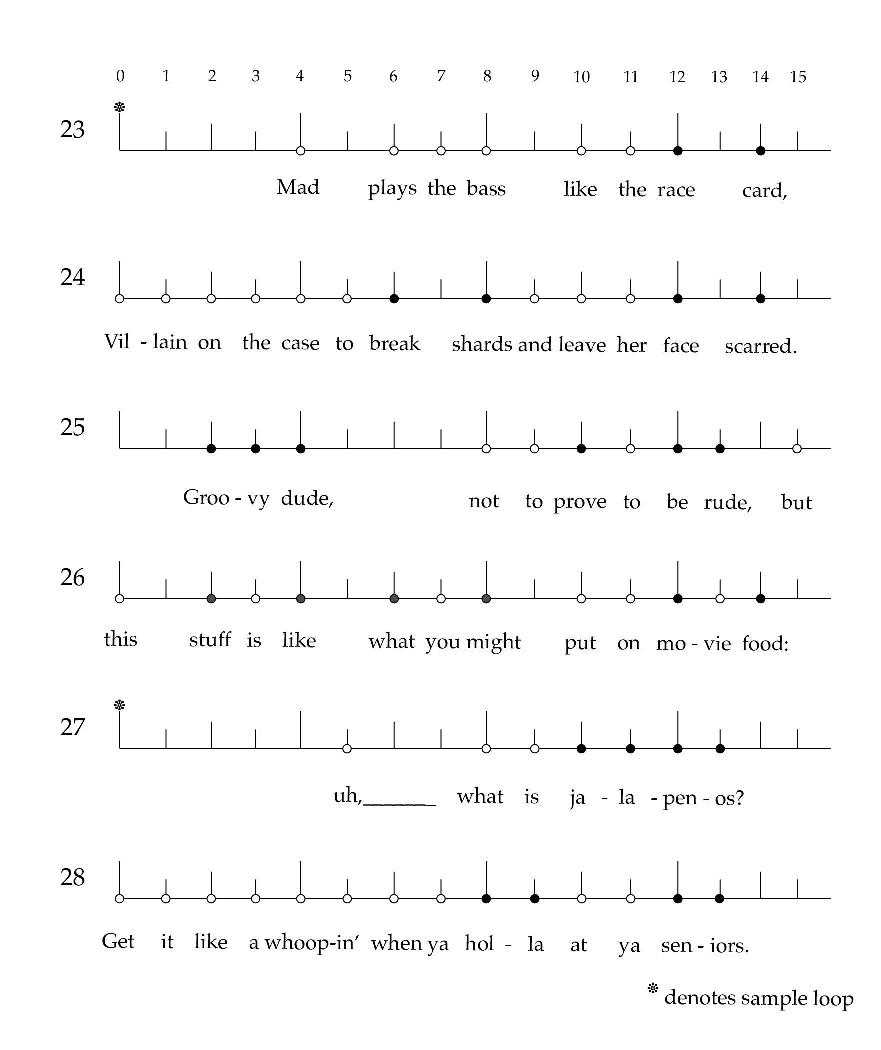
\includegraphics{images/figures/chp 03/059115greatdayfirstpivot.pdf}
        \caption{First pivot in Madvillain's ``Great Day,'' 0:59--1:15.}
        \label{fig:doomfirstpiv}
    \end{figure}

Over the next two bars, DOOM's flow increases in syntatic and rhythmic complexity, anticipating
the four-bar loop of the sample. Bars 25 and 26 increase the number of syllable onsets from 18 
to 22, as well as the  frequency, position, and syllable count of the rhymes. In the setup bar, 
DOOM creates an internal  rhyme with ``Groovy dude'' and ``prove to  be rude,'' each fitting 
within a durational segment of 2 from positions 2--4 and 10--12, respectively. In the punchline
, ``movie food'' once again restores the metric position of the end rhyme, preceded by two softer,
internal rhymes (``stuff is like'' with ``what you might'' falling between 2--4 and 6--8). Despite 
the increase in internal complexity, the  syntactic structure of these bars maintains regularity:
DOOM fits a sentence structured ``$x$, but $y$'' within the same time span as the previous setup 
and punchline.

My focus on the regular structure in the first four bars is important for establishing a connection
to the next four, two of which I transcribed as a part of Figure~\ref{fig:doomfirstpiv}. I perceive 
a semantic link in the content of bars 26 and 27 that allows DOOM to pivot to a new rhyme scheme but
in the process invites me as a listener to anticipate something different. It works as the setup for
a pivot rhyme but functions in a slightly different manner. My expectation at the end  of bar 26 is 
that DOOM is going to rap about butter: not only because I put butter on ``movie food,'' but also 
because he has done so twice already on the album up to this point.\footnote{
    DOOM refers to his ``buttery flow'' on ``Raid'' and Madlib's beats as ``so butter'' on ``All 
    Caps.''}
DOOM, of course, thwarts these expectations, positing ``uh\textellipsis what is jalapenos?'' as 
if  it were a botched  \textit{Jeopardy!} answer. He draws out a humorous semantic link between
these two bars, but rather than opting to construct a pivot rhyme with the word``butter'', he 
opts for jalapenos as an end rhyme for the following quatrain. With its final two syllables 
falling on positions 12 and 13, jalapenos ushers in a set of highly regular lines, each ending
with ``holla at ya  seniors,'' ``hashish fienda,'' and ``grass is greener'' in the same metric
positions.

    \begin{figure}[!p]
        \centering
        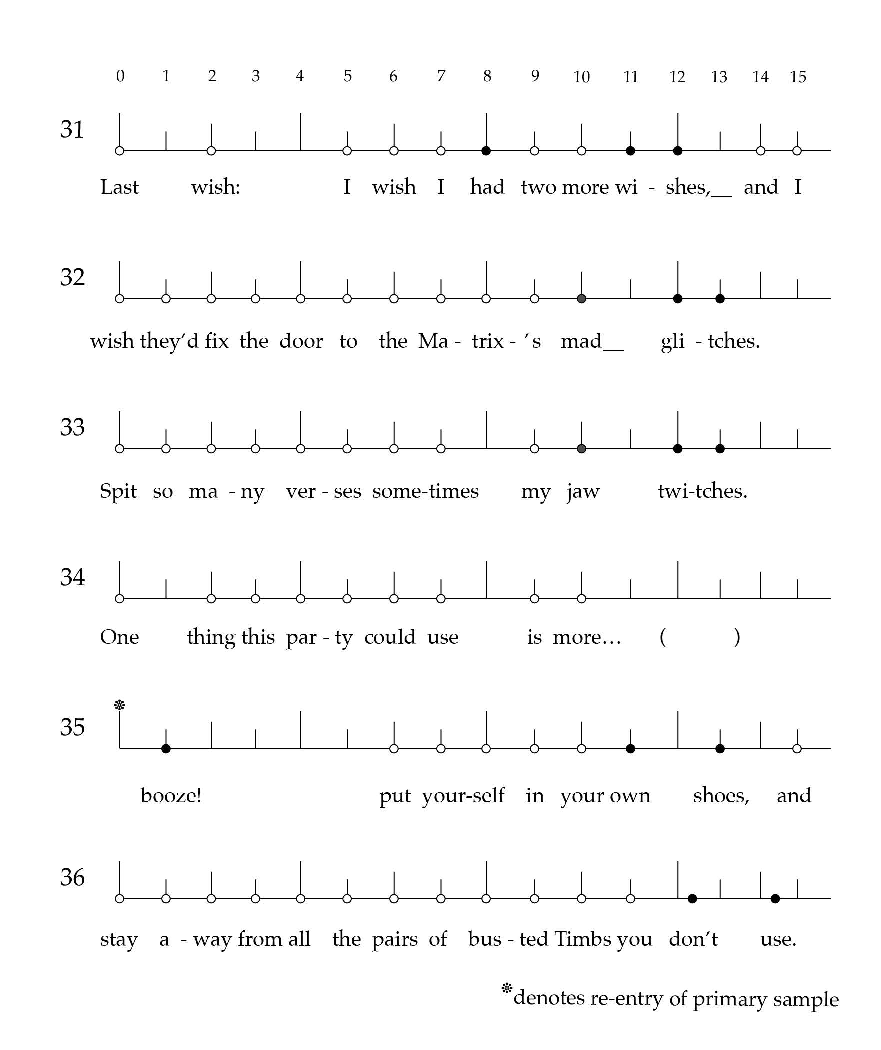
\includegraphics{images/figures/chp 03/121137greatdaysecondpivot.pdf}
        \caption{Second pivot in Madvillain's ``Great Day,'' 1:21--1:37.}
        \label{fig:doomsecondpiv}
    \end{figure}

DOOM's avoided pivot rhyme and the regularity of the subsequent quatrain provide crucial 
context for a similar moment between bars 34 and 35, an instance where I do apply the term
pivot rhyme. Figure~\ref{fig:doomsecondpiv} overviews a quatrain with a similarly regular
structure. ``Wishes''  falls on positions 11 and 12, displaced 1 position forward from the
ends of the two following  syntactic  closes: ``mad glitches'' and ``jaw twitches.'' The 
closely related structuring of the  middle bars of the quatrain set the listener up to hear:
``One thing this party could use is more\textellipsis booze.''And he makes that ellipsis 
audible! DOOM plays on listener expectations not only concerning rhyme structure, but also
their expectations concerning rap's ``topical stereotype:'' the humor in this instance
comes less from the fact that he implies the word ``bitches'' but that you expect that he
will say it.\footnote{
    My analysis of this moment varies slightly from Estelle Caswell's, who cites a 
    \textit{Pitchfork} reviewer's quotation that the ``hiliarity'' of this moment ensues
    from DOOM's non-sequitur (see \cite{estellecaswellRappingDeconstructedBest2016}).}
In effect, DOOM points the mic towards you at the end of this bar, asking you to examine
your listening expectations.

DOOM's patterning of flow, his regulating of syntactic structure, and his harnessing of
listener's expectations concerning rhyme lead into this moment; he crosses a barline, 
intentionally, yet again giving the listener a moment to expect one close to the phrase, 
before veering off in another direction. \textbf{Two more sentences here?}

%\clearpage
\phantomsection
\subsection*{\centering Armand Hammer and R.A.P. Ferreira's ``Dead Cars''}
\addcontentsline{toc}{subsection}{Armand Hammer and R.A.P. Ferreira's ``Dead Cars''}

Armand Hammer\textemdash the name given to the collaboration between billy woods and
ELUCID\textemdash is a flagship act on the roster of the New York based underground 
label Backwoodz Studioz.\footnote{
    \textbf{cite reviews?}}
The track ``Dead Cars'' from the 2019 LP \textit{Shrines} features production from 
Kenny Segal, as well as a feature verse from R.A.P. Ferreira\textemdash two premiere 
artists from Ruby Yacht, an underground hip-hop label for which Ferreira serves as 
the owner-operator. In short, as a track, it features some of the underground artists
who exist at the center of my conception of the genre, whose techniques as performers
deeply inform my construction of underground methodology.

The track features several short verse-parts delivered by each of the emcees. Counting
at 64 bpm, ELUCID, Ferreira, woods  rap for eight bars at a time, comparable to how
jazz musicians may trade fours on a jazz tune. Ferreira's feature verse enters after
ELUCID's second eight-bar section, accompanied by a drastic change in the musical 
texture. As Segal layers out the drum loop, he recomposes the orginal synth-texture
chord loop: a Fender Rhodes strikes chords on the downbeats and samples reversed audio
to construct a melodic line in between downbeats. Figure~\ref{fig:roryclosingfrag} 
transcribes the last six bars of Ferreira's verse, two bars prior to the drum's
re-entry.

    \begin{figure}[!htp]
        \centering
        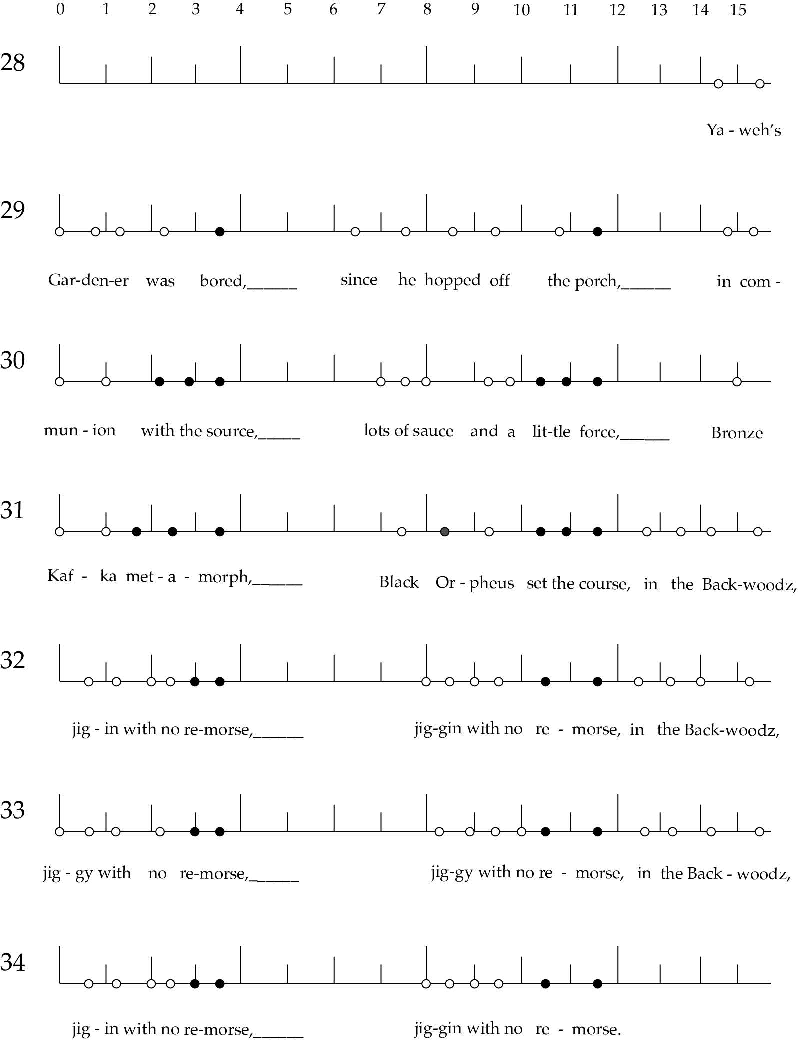
\includegraphics{images/figures/chp 03/144206deadcarsendfrag.pdf}
        .\caption{Closing fragmentation in ``R.A.P. Ferreira's ``Dead Cars,'' 1:44--2:06.}
        \label{fig:roryclosingfrag}
    \end{figure}

Without a drum loop's articulation of a clear metrical hierarchy, Ferreira lets his text
float around freely in micro-rhythmic space; however, Ferreira uses rhyming syllables as
an anchor for the more lax placement of the intervening syllables. He places the end of 
his rhyming in slight anticipation of positions 4 and 12, where the snare drum often hits
in a drum loop.\footnote{
    According to Ohriner, orientation around these two beats is foundational to the 
    construction of the boom-bap texture pervasive in hip-hop beats (see his discussion
    of A\$AP Rocky's ``Purple Swag:  Chapter 2'' in 
    \autocite[18]{mitchellohrinerFlowRhythmicVoice2019}). My decision to mark out what 
    seems to be a slower, half-time tempo in ``Dead Cars'' is based on this orientation
    normalizes my hearing of the vocal sections as verse-parts rather than full verses.}
This rhyme structure may seem commonplace, but his choice to continue doing so without 
the drum loop strictly articulating them is important for orienting a listener in the 
sparse musical texture.

When, in bar 31, the drums do re-enter, Ferreira stops rapping new text. Syntactically,
his remaining four bars only rely on what I hear as two units: ``Bronze Kafka metamorph, 
Black Orpheus set the course / in the Backwoodz, jiggin' with no  remorse.''\footnote{
    My hearing of the first bar as a full syntactic unit is in part due to his rapping 
    of it within the space of one bar, but it has some semantic justification. I hear
    ``Bronze Kafka'' and ``Black Orpheus'' as two epithets the emcee gives 
    himself\textemdash the first a play on the author's name; the second, a nod to the
    1959 Brazilian film of the same name.}
The second of the two, a shoutout to the label to which his host emcees are signed, serves
as the textual focus of his shift into a more improvisatory form of vocal delivery. Maintaining
the rhythmic position of the final rhyming word ``remorse,'' Ferreira shifts the text around
in his three repetitions of the phrase: the verb-form \textit{jiggin'} becomes the adjective
\textit{jiggy} as Ferreira shifts the metric placement of the first syllable to on the beat
in bar 32, position 1 and behind the beat in position 8. Before cycling back to a near direct
repetition in bar 33, he slightly accelerates ``Backwoodz'' from its original position, though
still completing his statement as a pickup to the downbeat of the next bar.

For a listener familiar with Ferreira's style, the mode of delivery into which he shifts
functions as signposting that the verse is coming to a close. When he shifts into a textual
delivery that is more fragmented, repeated, and rhythmically varied (in this instance, while
delivering his shout out to the other emcees for hosting him), he is fragmented and repeated
text to tell an audience that he is finished rapping; therefore, I refer to this structuring 
device as \emph{closing fragmentation}.

Ferreira's technique relates to methods of delivering text that are used to signal a change
in formal sections theorized by Ben Duinker. In particular, Duinker identifies fragmentation
and repetition as signs that the rapper is no longer delivering a verse but instead either a
hook or a looser organized vocal-section.\footnote{
    \autocite[98--101]{benduinkerSongFormMainstreaming2020}. Duinker's definition of hook is 
    discussed on p.~\pageref{duinkerhookdef}. His ``looser-organized'' sections function like
    a catch all category; he includes ``ad-hoc, ametric vocals, skits, or\textellipsis [rapping]
    that doesn't function like a verse or hook'' as typical in this section-type.}
Constructed from examining form in mainstream hip-hop, Duinker's categories break down due to
Ferreira's use of the technique within the verse as a formal unit. The rhyme scheme matches of
the fragmented units matches that of the verse immediately preceding it (so too the metric 
placement of its rhymes). And though the phrase's semantic content may be construed as a kind
of ``hype'' vocal that Duinker identifies, Ferreira imbues them with a structural function that
cannot be located outside the verse: signalling its close. Closing fragmentation, then, become
s a valuable way to describe an emcee's use of fragmentation and repetition more with a new 
categorical purpose. 

In my listening, this technique most prominently occurs in Ferreira's catalog. His influence, 
however, can perhaps be traced in the use of this technique by other emcees in his satellite:
in particular, other members of the Ruby Yacht crew including Pink Navel and S.AL have taken 
to the technique when constructing their own rhymes. Perhaps most telling that this technique
is more than just Ferreira's  idiosyncrasy: each of the verse-parts that precede Ferreira's on
``Dead Cars'' end with some form of closing fragmentation as well.

%\clearpage
\section{Performance Techniques}
\phantomsection

An emcee's performance of their rhymes demands a slightly different approach to the transcription
of a musical object, one which can account more clearly for pitched elements and their interrelation
in a musical texture. Ohriner's monograph on flow does not uniformly employ a method of transcription
that accounts for verses in pitch-space, later works of his develop a contour-graph method of showing
changes of pitch broadly over the range of G2--G4 with gridlines.\footnote{
    \textbf{Ohriner, 2019, analysing pitch of the rapping voice, 418--419.}}

My approach to representing pitch marks a point of departure from Ohriner's, likely due to conflicting
readings of the imperatives about transcription discussed in the prior section. He takes Agawu's
admonitions to use transcription as a means of illuminating musical practice as a drive to look beyond
the confines of standard notation. On the contrary, I adamantly believe Agawu suggests music theorists 
should use standard notation \textit{creatively} to articulate a complex picture of its sameness and 
difference from familiar repertory within our sphere of discourse. It is for this reason that my 
transcriptions in this section harness standard notation diacritically, transcribing rap flows pitched
in relation to themselves and other musical elements.\footnote{
    Such an approach to notation has precedence in \textbf{Robert Komaniecki, Vocal Pitch in Rap Flow} and 
    \textbf{Martin Connor, Musical Artistry of Rap}.}

\subsection*{\centering R.A.P. Ferreira's ``NONCIPHER''}
\addcontentsline{toc}{subsection}{R.A.P. Ferreira's ``NONCIPHER''}

If one were to look through R.A.P. Ferreira's catalog on any major streaming platform, they would
guess that the 2020 LP \textit{Purple Moonlight Pages} is an artistic debut, but this is not case.
In reality, Ferreira's career spans the entire preceding decade with a full catalog of releases under
various monikers, the most prominent of these being Milo. He ties the decision to switch to his own
name closely to the concept of identity: ``my name is rory allen phillip ferreira. and after 9 years
pro rapping i'm confident enuff to put it on what i make. i never knew who milo was.''\footnote{
    \textbf{Tweet on May 31, 2019.}}
Ferreira's statement\textemdash that he now raps in a way deserving of his given name rather than 
a chosen alias\textemdash speaks to the intentional curation of identity that takes place within 
underground hip-hop and therefore demonstrates that his musical style as ``R.A.P. Ferreira'' is 
something worth investigating.

Along with his persistent use of closing fragmentation noted above, one element of his music that
manifests in musical performance is his vocal mimesis of elements of the musical texture. 
Figure~\ref{fig:rorymimesis} examines instances in the second verse of ``NONCIPHER'' where Ferreira
delivers his verse in a dialogue with the alto saxophone, live-tracked by Aaron Shaw.
    \begin{figure}[!t]
        \centering
        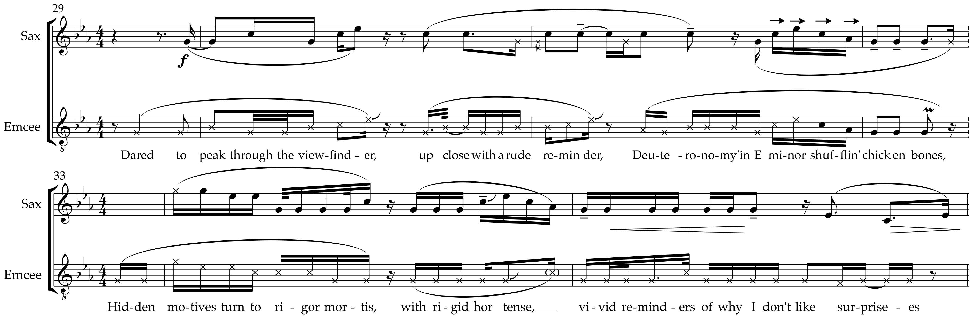
\includegraphics{images/figures/chp 03/120137nonciphermimesis.pdf}
        \caption{Mimesis in R.A.P. Ferreira's ``NONCIPHER,'' 1:20--1:37.}
        \label{fig:rorymimesis}
    \end{figure}
Immediately following a verse that ends in closing fragmentation, Ferreira and Shaw both anticipate
m.~30 with syncopated entrances to the second verse. Although Ferreira cuts across the saxophone's 
phrase beginnings and endings later, his first clause of text (``Dared to peak through the viewfinder'')
aligns with Shaw's performance in both rhythmic placement and pitch contour. Shaw's lick also informs
his delivery of the subsequent clause (``up close with a rude reminder''). As Shaw presses on, 
Ferreira approaches the downbeat of m.~30 in close approximation of Shaw's performance, singing the 
phrase ``shufflin' chicken bones'' with the same melodic inflection as Shaw, adding a shake to his 
delivery at the phrase's end.

After a brief departure from the mimicking the saxphone, Ferreira once again locks in with Shaw at
the onset of m.~34. Traversing into a higher register to mimic the saxophone's G5, he raps ``[hidden]
motives turn to rigor mortis'' in a related but staggered descent from Shaw's outlining of a C minor
triad. The lick outlining G to C (m.~34, beat 2) delivered by Shaw gives Ferreira another contour
to mimic within the beats that immediately follow: ``rigid hortense'' ends with a shadow vowel that
inflects upwards, and ``vivid reminders'' places its final syllable in a higher register than those
which immediately precede it. In general, Ferreira uses mimesis at this verse's beginning to align 
his vocal performance to  the saxophone line.

The rhetorical value of this performance technique is two-fold as it relates to Ferreira's identity 
as an underground emcee. That he draws us into the saxophone melody as a demonstration of his own 
musicality, marking his voice as a musical participant in the whole texture. The ``beat'' in this 
verse section is not simply something happening around or behind Ferreira's flow; instead, he puts 
himself on display \emph{as} a listener, encouraging a similar engagement \emph{from} the listener.
Moreover, this reorders the hierarchy of the rap song as a musical object: the emcee's performance
does not supersede any instrumental stream simply because of its use of text. Instead, the text is
fused to the music surrounding it.

%\clearpage
\phantomsection
\subsection*{\centering Moor Mother,  billy woods, and ELUCID's ``Tiberius''}
\addcontentsline{toc}{subsection}{Moor Mother, billy woods, and ELUCID's ``Tiberius''}

An underground emcee's fusion of text to music also informs my processing as a performance technique. 
Underground emcees are often responsible not only the construction and performance of their own text 
but often the means by which their voice is captured in the recording process. Although a quality 
microphone and some compression, EQ, and reverb does the trick for many emcees, others such as Moor 
Mother explore a wider range of possibility for what exactly vocal tracking of a rap verse entails.
Her verse on the track ``Tiberius'' from the collaborative LP \textit{Brass} (2020) with billy woods
illustrates her more maximal approach to fitting her voice in the musical texture.

Moor Mother's use of multitracking and effects processing demands a wider conception of the idea of a
unitary ``vocal stream'' occurring the beat. Figure~\ref{fig:moormotherprocess} details the components
of her vocal tracking in the first fifteen bars of her verse. Entering on the heels of ELUCID's final 
bar, she repeats the text he just delivered (``It's me dummy!'') as a pivot into her own verse. The 
channel on which this verse enters (Moor Mother II in the figure) proves to be a secondary, ad-lib 
track, as a more-prominent vocal  enters in the next bar (Moor Mother I in the figure). This vocal 
channel bifurcates into a lower, primary layer of vocals and one created with a transposition effect,
sounding around a fifth higher than the primary layer, represented by diamond-head notation in 
the figure.

\begin{figure}[!p]
    \centering
    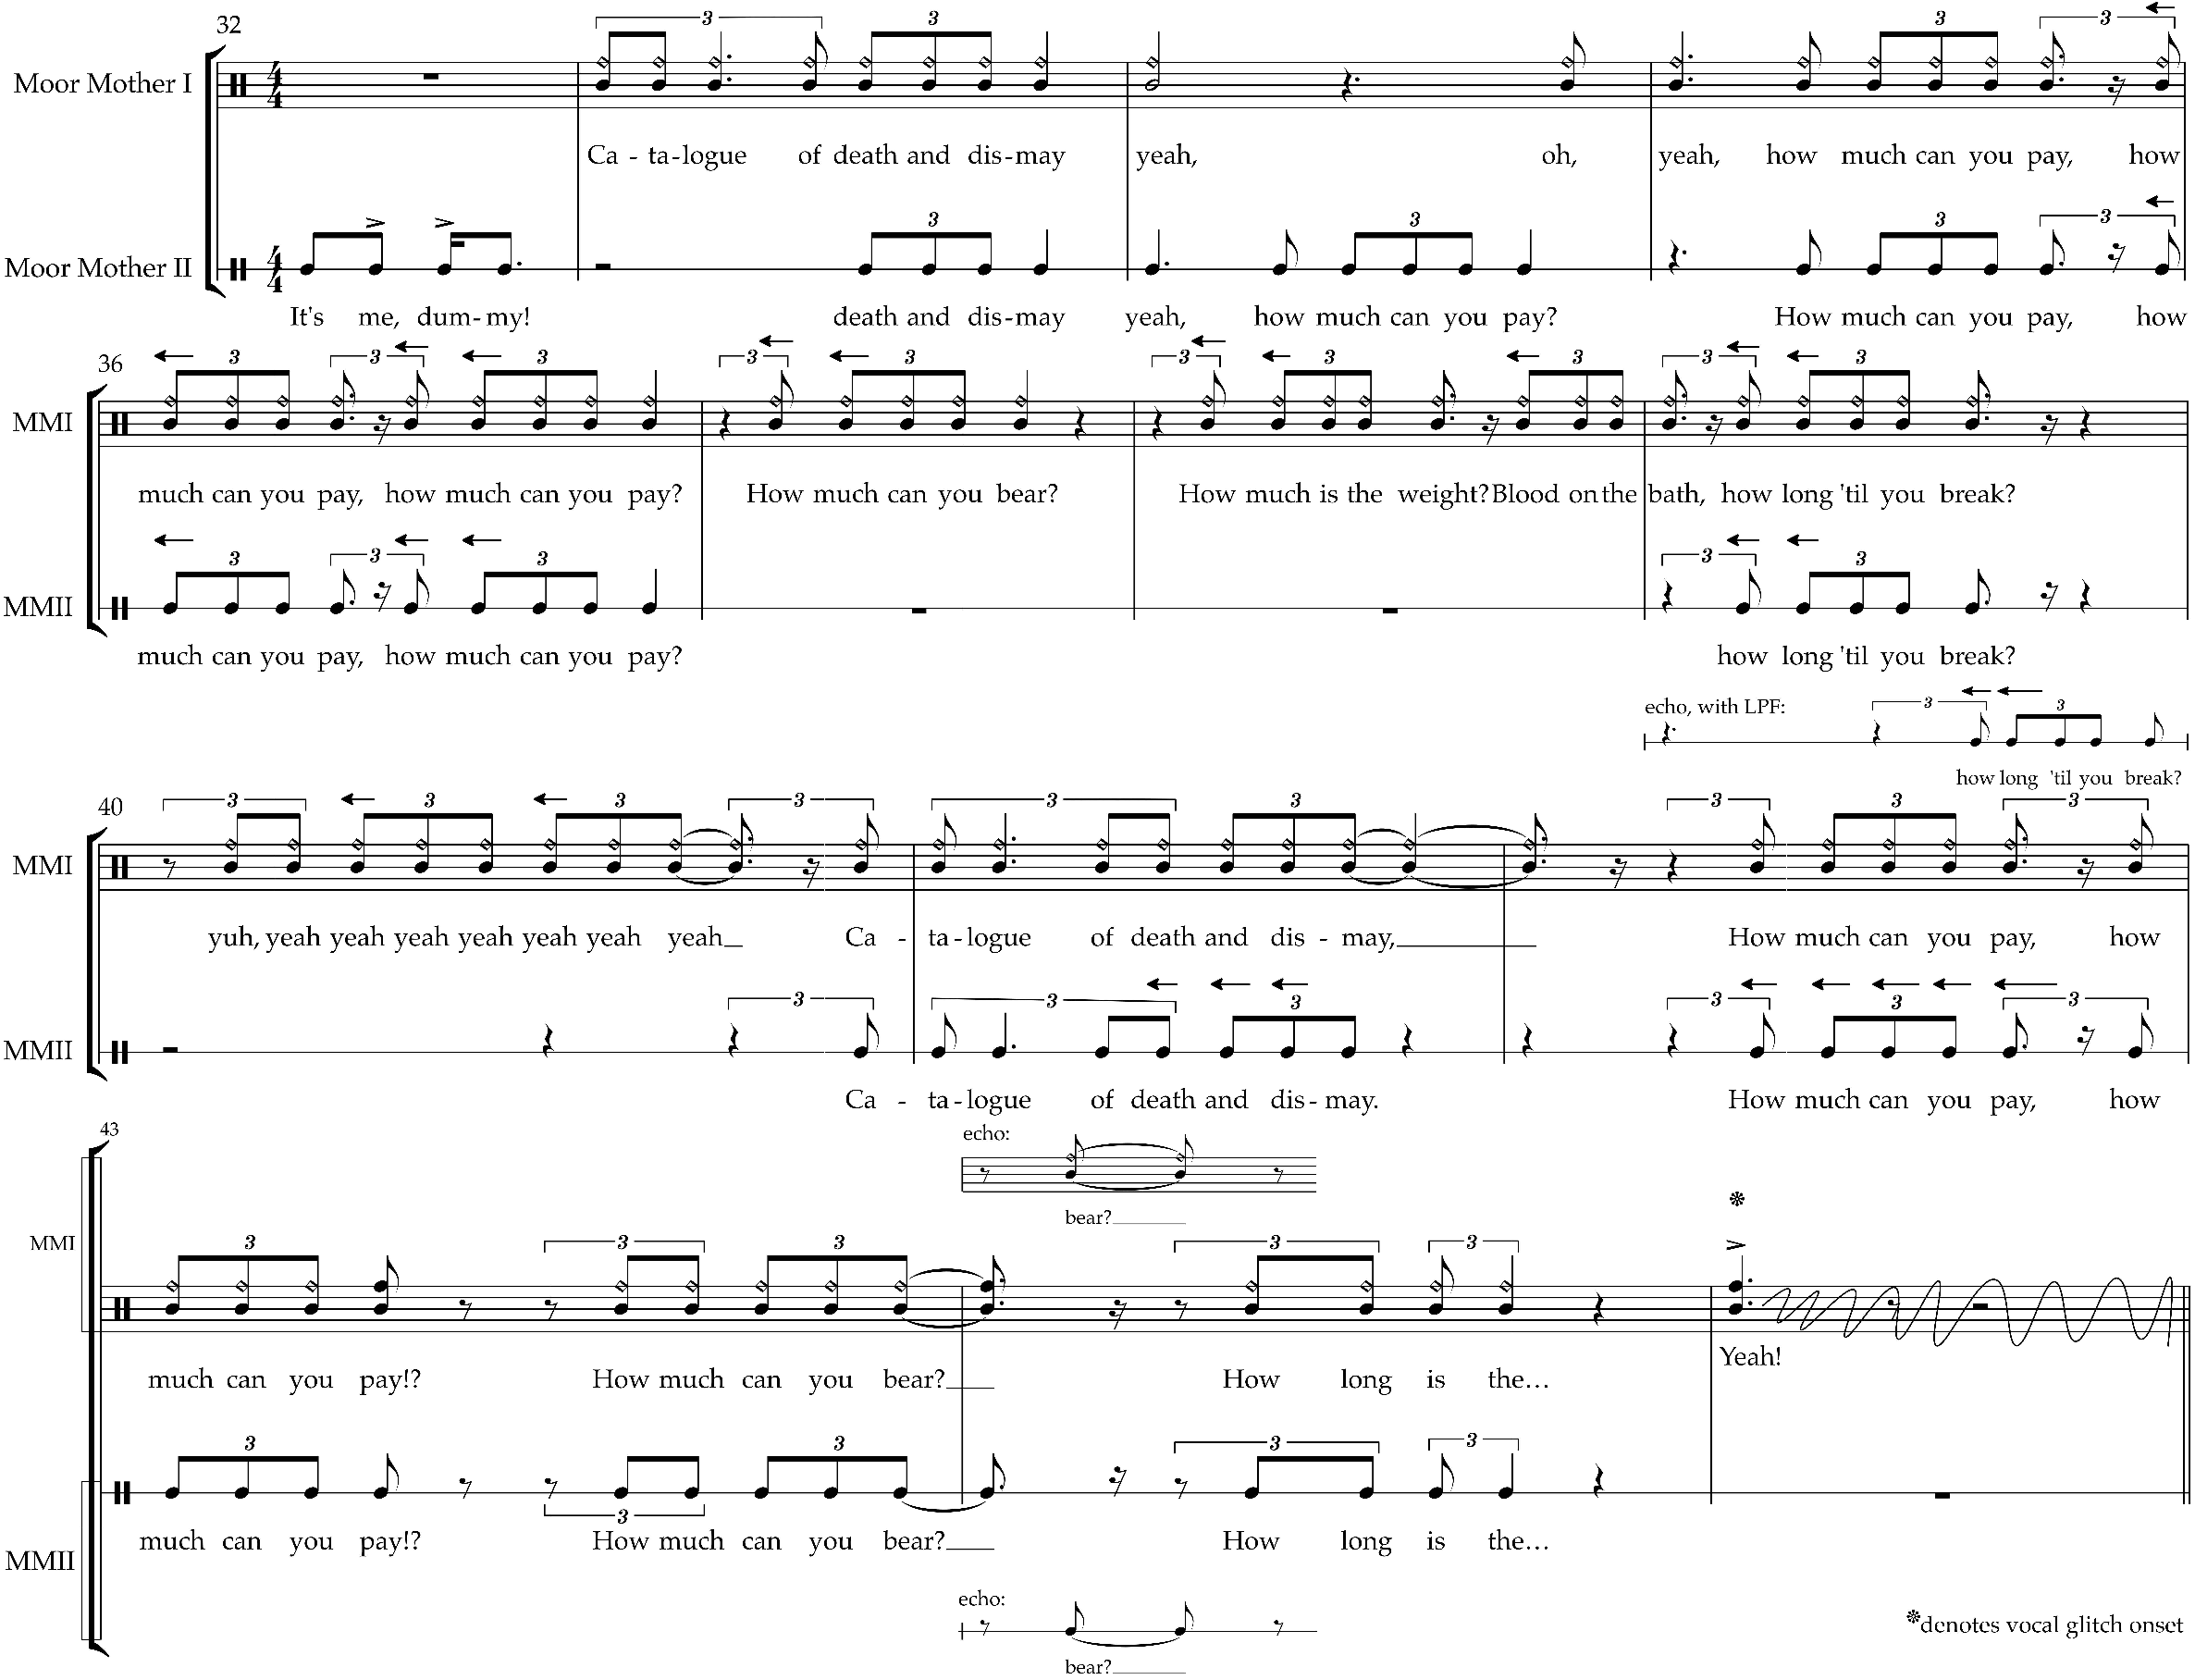
\includegraphics[width=\textwidth]{images/figures/chp 03/107136tiberiusprocessing.pdf}
    \caption{Vocal processing in Moor Mother and billy woods' ``Tiberius,'' 1:07--1:37.}
    \label{fig:moormotherprocess}
\end{figure}

Moor Mother uses these two vocal channels to deliver the first twelve bars of her verse: a series
of questions rapped in a triplet flow pattern that slightly anticipates the beat. The hurried, 
harsh delivery of her verse crests in mm. 39--41, where she shifts the delivery far enough forward
in the grove that the first eighth-note of her tuplet on the text ``catalogue of death and dismay''
syncopates before the downbeat. In the bar before this shift, she adds an echo of the triplet ad-lib
on ``how long `til you break,'' panned hard left in the mix and processed with a low-pass EQ filter
to diminish its prominence in the mix; the echoes shown in Figure~\ref{fig:moormotherprocess} on
an ossia staff below Moor Mother II.

In the following three measures, Moor Mother's use of processing helps to articulate an oncoming 
boundary within her verse\textemdash a transition to a flow with new rhythmic gestures and articulations.
Repeating text in a new rhythmic position, she arrives at the question ''how much can you bear?'' 
in slight anticipation of the downbeat of m.~44. Another echo repeats the text ``bear'' mid-measure,
this time in both vocal channels. Trailing off during the final question ``How long is the (wait),''
she delivers a guttural ``yeah!'' exclamation on the following downbeat.

%\clearpage
A sonic marker of the transition to the rest of the verse, this moment is marked out with effects 
processing throughout the texture: the synth, which had dropped out upon the textual repeat, now
re-enters with a wash of noise while Moor Mother's textual exclamation is extended through the 
use of a glitch-like delay. The delay used in this instance increases the frequency of signal 
repetitions at the same time that it extends the feedback time for the loop, letting the sound
of the ``Yeah!" more quickly double up on itself and extend across the remainder of the bar. This
timbre is also heightened in the mix, as the delayed signal ``ping-pongs'' back and forth from 
the right to left audio channels.

At this point, the function of the exclamation is no longer textual in the way any of the questions
preceding it have been. Through the use of glitch, the audio of Moor Mother's voice carries less 
semantic weight and functions more abstractly as a sound, receding into the mix as she begins the
next section of her verse. But at the same time, Moor Mother's treatment of the audio of her voice(s)
throughout the excerpt demonstrates that her vocals have more than one function. Certainly, they carry
the text, and the text carries semantic value, perhaps even a poetic meaning for the listener. But the
use of several distinct and overlapping vocal signals, each with its own performative subtleties 
stratifies the concept of the ``emcee's voice'' within the musical texture. Her particular approach
heightens the voice to become \emph{synthetic}; each layer's treatment could be likened to several
oscillators used to create a synthesizer patch. Rather than approaching vocal treatment as 
contrapuntally distinct lines, Moor Mother's audio processing creates heterogeneity within a single
``line'' of music, and likens its role to any other multitracked musical element in the mix.